

\documentclass[12pt]{article}

%%% These are some packages that are useful
\usepackage{amsfonts, lipsum}
\usepackage{amsmath,amssymb, amscd,amsbsy, amsthm, enumerate}
\usepackage{titlesec, setspace,verbatim, multicol}
\usepackage[top=1in, bottom=1in, left=.45in, right=.45in]{geometry}
\usepackage[unicode]{hyperref}
\usepackage{tikz, pgfplots, xcolor, fancyhdr}
\usepackage{listings}
\usepackage{xcolor}
\usepackage[framemethod=TikZ]{mdframed}

%%% Page formatting
%\setlength{\headsep}{30pt}
\setlength{\parindent}{0pt}
\setlength{\textheight}{9in}

%%% Header and Footer Info
\pagestyle{fancy}
\fancyhead[L]{{\large Free Time - \textbf{Differential Equation Analysis}}}
\fancyhead[C]{}
\fancyhead[R]{Name: Antonius Torode}
\fancyfoot[L]{MSU}
\fancyfoot[C]{\thepage}
\fancyfoot[R]{\LaTeX}

%%% These define our question environment and help number things correctly
\theoremstyle{definition}
\newtheorem{thm}{Theorem}
\newtheorem{question}[thm]{Question}
\newtheorem{prop}[thm]{Proposition}
\newtheorem{lem}[thm]{Lemma}
\newtheorem{DEF}[thm]{Definition}
\newtheorem{rem}[thm]{Remark}

%%% This defines the solution environment for you to write your solutions
\newenvironment{soln}
{\let\oldqedsymbol=\qedsymbol
	\renewcommand{\qedsymbol}{$ $}
	\begin{proof}[\bfseries\upshape \color{blue}Solution]\color{blue}}
	{\end{proof}
	\renewcommand{\qedsymbol}{\oldqedsymbol}}

%%% This defines the note environment for you to write your notes
\newenvironment{note}
{\let\oldqedsymbol=\qedsymbol
	\renewcommand{\qedsymbol}{$ $}
	\begin{proof}[\bfseries\upshape \color{blue}Note]\color{red}}
	{\end{proof}
	\renewcommand{\qedsymbol}{\oldqedsymbol}}


%%% These are some shortcuts that are handy
\def\real{{\mathbb R}}
\def\Natural{\mathbb{N}}
\def\dx{\textnormal{dx}}
\def\dy{\textnormal{dy}}
\def\dz{\textnormal{dz}}
\def\dt{\textnormal{dt}}
\def\ds{\textnormal{ds}}
\def\dw{\textnormal{dw}}
\def\Re{\textnormal{Re}}
\def\Im{\textnormal{Im}}
\def\exp{\textnormal{exp}}
\def\interior{\textnormal{interior}}
\def\al{\alpha}
\def\del{\delta}
\def\Del{\Delta}
\def\gam{\gamma}
\def\Gam{\Gamma}
\def\Om{\Omega}
\def\ep{\varepsilon}
\def\lam{\lambda}
\def\rational{{\mathbb Q}}
\def\integer{{\mathbb Z}}
\def\Q{{\mathbb Q}}
\def\Z{{\mathbb Z}}
\def\N{{\mathbb N}}
\def\R{{\mathbb R}}
\def\grad{\nabla}
\def\C{\mathcal C}
\def\P{\mathcal P}
\def\T{\mathcal T}
\def\I{\mathcal I}
\newcommand{\abs}[1]{\left| #1 \right|}
\newcommand{\inner}[1]{\langle #1 \rangle}
\newcommand{\norm}[1]{\left\lVert#1\right\rVert}
\newcommand{\spanvect}{\textnormal{span}}
\newcommand{\union}{\cup}
\newcommand{\Union}{\bigcup}
\def\intersect{\cap}
\def\Intersect{\bigcap}

\DeclareMathOperator*{\Limsup}{LIMSUP}



\lstset { %
	language=C++,
	backgroundcolor=\color{black!5}, % set backgroundcolor
	basicstyle=\footnotesize,% basic font setting
}

\title{The Art of Problem Solving: \\Analysis of Differential Equations}
\date{\today}
\author{Antonius Torode, Michigan State University, \\ Written in \LaTeX}

\numberwithin{equation}{section}
\setlength{\columnsep}{.5cm}
\setlength{\columnseprule}{1pt}
\def\columnseprulecolor{\color{black}}




%theorem
\newcounter{theo}[section] \setcounter{theo}{0}
\renewcommand{\thetheo}{\arabic{section}.\arabic{theo}}
\newenvironment{theo}[2][]{%
	\refstepcounter{theo}%
	\ifstrempty{#1}%
	{\mdfsetup{%
			frametitle={%
				\tikz[baseline=(current bounding box.east),outer sep=0pt]
				\node[anchor=east,rectangle,fill=blue!20]
				{\strut Theorem~\thetheo};}}
	}%
	{\mdfsetup{%
			frametitle={%
				\tikz[baseline=(current bounding box.east),outer sep=0pt]
				\node[anchor=east,rectangle,fill=blue!20]
				{\strut Theorem~\thetheo:~#1};}}%
	}%
	\mdfsetup{innertopmargin=10pt,linecolor=blue!20,%
		linewidth=2pt,topline=true,%
		frametitleaboveskip=\dimexpr-\ht\strutbox\relax
	}
	\begin{mdframed}[nobreak=true]\relax%
		\label{#2}}{\end{mdframed}}
%%%%%%%%%%%%%%%%%%%%%%%%%%%%%%






%Lemma
\newcounter{lemm}[section] \setcounter{lemm}{0}
\renewcommand{\thelemm}{\arabic{section}.\arabic{lemm}}
\newenvironment{lemm}[2][]{%
	\refstepcounter{lemm}%
	\ifstrempty{#1}%
	{\mdfsetup{%
			frametitle={%
				\tikz[baseline=(current bounding box.east),outer sep=0pt]
				\node[anchor=east,rectangle,fill=green!20]
				{\strut Lemma~\thelem};}}
	}%
	{\mdfsetup{%
			frametitle={%
				\tikz[baseline=(current bounding box.east),outer sep=0pt]
				\node[anchor=east,rectangle,fill=green!20]
				{\strut Lemma~\thelem:~#1};}}%
	}%
	\mdfsetup{innertopmargin=10pt,linecolor=green!20,%
		linewidth=2pt,topline=true,%
		frametitleaboveskip=\dimexpr-\ht\strutbox\relax
	}
	\begin{mdframed}[]\relax%
		\label{#2}}{\end{mdframed}}
%%%%%%%%%%%%%%%%%%%%%%%%%%%%%%
%Definition
\newcounter{defn}[section] \setcounter{defn}{0}
\renewcommand{\thedefn}{\arabic{section}.\arabic{defn}}
\newenvironment{defn}[2][]{%
	\refstepcounter{defn}%
	\ifstrempty{#1}%
	{\mdfsetup{%
			frametitle={%
				\tikz[baseline=(current bounding box.east),outer sep=0pt]
				\node[anchor=east,rectangle,fill=gray!20]
				{\strut Definition~\thedefn};}}
	}%
	{\mdfsetup{%
			frametitle={%
				\tikz[baseline=(current bounding box.east),outer sep=0pt]
				\node[anchor=east,rectangle,fill=gray!20]
				{\strut Definition~\thedefn:~#1};}}%
	}%
	\mdfsetup{innertopmargin=10pt,linecolor=gray!20,%
		linewidth=2pt,topline=true,%
		frametitleaboveskip=\dimexpr-\ht\strutbox\relax
	}
	\begin{mdframed}[nobreak=true]\relax%
		\label{#2}}{\end{mdframed}}


%%% Document Starts now
\begin{document}
\maketitle
\begin{center}
	\vspace{2cm}
	%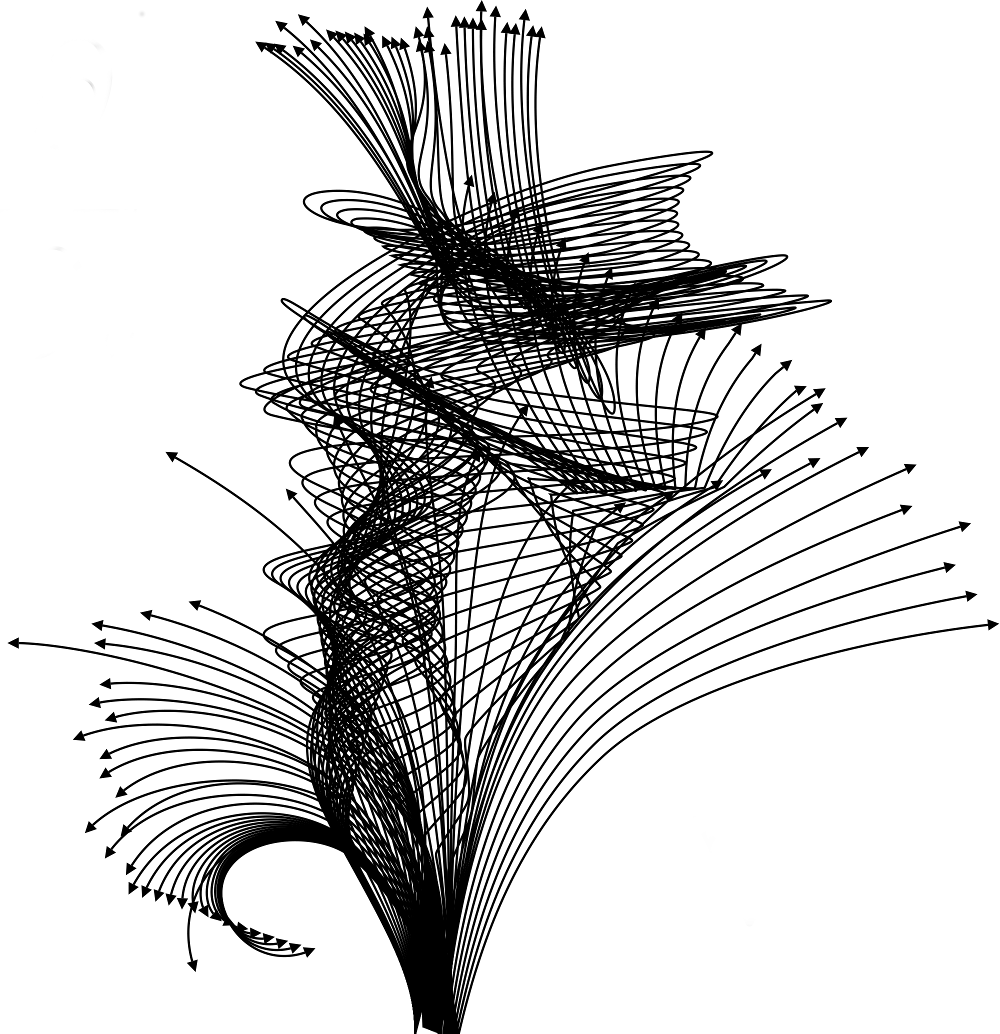
\includegraphics[scale=0.3]{diff-eq2.jpg}
	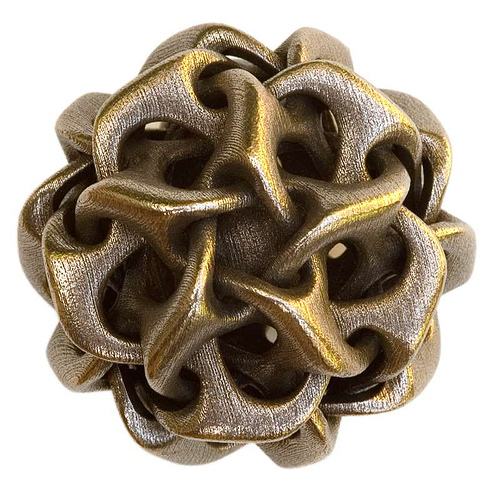
\includegraphics[scale=0.6]{diff-eq3.jpg}
\end{center}
\newpage

\begin{abstract}
	This document is intended for my own personal learning process. The ideas are in no specific order, but is intended for me to write my thoughts on the subject of differential equations down in a concise manner in a similar location. Anyone may freely distribute this document or take any individual part of the document to share with others but please provide proper credit to the author. The format of this will also be quite strange as I will be working out ideas and them writing a "theorem" based on it, with no proof for these theorems as the proof would be found in the prior work. All work done in this document is completely my own except when stated otherwise.
\end{abstract}
\tableofcontents


















\newpage
\section{Useful Concepts, Proofs, and key Ideas}
This section is mainly to help show and prove in between steps and useful ideas that will be used later. The summation operator will be used extensively and it would be a good idea to have some rules for using it in a concise and efficient manner. To begin with, a useful idea is to sum each term of the binomial coefficient which will be used later. First, by definition of the binomial coefficient, we can write
\begin{align}
{{n}\choose{k}}&=\frac{n!}{(n-k)!k!}\\
&=\frac{(n-1)!n}{(n-k)!k!}\\&
=\frac{(n-1)!n-k(n-1)!+k(n-1)!}{(n-k)!k!}\\
&=\frac{(n-1)!(n-k)}{(n-k)!k!}+\frac{k(n-1)!}{(n-k)!k!}\\
&=\frac{(n-1)!}{(n-1-k)!k!}+\frac{(n-1)!}{(n-k)!(k-1)!}\\&={{n-1}\choose{k}}+{{n-1}\choose{k-1}}\\
&\equiv {{m}\choose{k}}+{{m}\choose{k-1}}, \textrm{ with }m=n-1.
\end{align} 
Observe for a moment that (1.6) can be expanding even further. By the same process of going from (1.1) to (1.6), we can say
\begin{align}
{{n-1}\choose{k-1}} = {{n-2}\choose{k-1}}+{{n-2}\choose{k-2}}.
\end{align}
Thus, (1.6) becomes
\begin{align}
{{n}\choose{k}}={{n-1}\choose{k}}+{{n-2}\choose{k-1}}+{{n-2}\choose{k-2}}.
\end{align}
If we continue this pattern, we can see that we can write the binomial coefficients as a sum of binomial coefficients with incrementally decreasing numerators (i.e n!, (n-1)!, (n-2)!,...). This gives
\begin{align}
{{n}\choose{k}}&={{n-1}\choose{k}}+{{n-2}\choose{k-1}}+{{n-3}\choose{k-2}}+\cdots+{{1}\choose{k+2-n}}+{{0}\choose{k+1-n}} \\
&=\sum_{i=1}^{n}{{n-i}\choose{k+1-i}} \\
&=\sum_{i=0}^{n-1}{{n-1-i}\choose{k-i}}.
\end{align}
Note that we stop the above sequence when the numerator of our factorial sequence has reached zero. If we were to continue the sequence, we would end up having negative factorials in our numerator which would make evaluating the binomial coefficient at that term and the following terms difficult. However, if we happen to have a smaller $k$ than $n$, it may be such that we end up having negative $k$ numbers. This is ok for now, as it will lead to complex infinities in the denominator of our binomial coefficient expressions hence making those terms zero. This will be demonstrated later. Now, suppose we claim that for all $n\in \mathbb{N}$, that
\begin{align}
\sum_{i=0}^{n}{{n}\choose{i}} =\sum_{i=0}^{n}\frac{n!}{(n-i)!i!}= 2^n.
\end{align}
We can then do a proof by induction to prove this is in fact true for all $n,k \in \mathbb{N}$. First, we can see checking the base cases hold as when $n=0$, we have $1=1$, when $n=1$, we have $2=2$, and when $n=3$ we have $4=4$. Next, let's assume for any $n=k$ that (1.1) holds true. Now, if we let $n=k+1$ we have from the left hand side of our expression,
\begin{align}
\sum_{i=0}^{k+1}{{k+1}\choose{i}}&={{k+1}\choose{0}}+{{k+1}\choose{1}}+\cdots+{{k+1}\choose{k}}+{{k+1}\choose{k+1}} \\
&={{k}\choose{0}}+{{k}\choose{-1}}+{{k}\choose{1}}+{{k}\choose{0}}+\cdots+{{k}\choose{k}}+{{k}\choose{k-1}}+{{k}\choose{k+1}}+{{k}\choose{k}}\\
&=2{{k}\choose{0}}+2{{k}\choose{1}}+\cdots+2{{k}\choose{k-1}}+2{{k}\choose{k}}\\
&=2\sum_{i=0}^{k}{{k}\choose{i}}\\
&=2(2^k)\\
&=2^{k+1}.
\end{align}
Therefore, we can see that for $n=k+1$ that equation (1.8) holds true, and thus we conclude by induction that (1.8) holds for all $n\in\mathbb{N}$. Note that in the above proof, we made use of ${{k}\choose{k+1}}={{k}\choose{-1}}=0$. If we were to evaluate each of these using the definition of the binomial coefficient above we may notice a slight issue. Suppose we try to evaluate ${{n}\choose{-1}}$. Using the definition from (1.1), we would have
\begin{align}
{{n}\choose{-1}}&=\frac{n!}{(n-(-1))!(-1)!}\\&=\frac{n!}{(n+1)!(-1)!} \\
&=\frac{n!}{(n)!(n+1)(-1)!} \\
&=\frac{1}{(n+1)(-1)!}.
\end{align}
From above, we have a negative factorial in hte denominator of our expression. Since this is not easily determined as a positive integer factorial would be, we will need to expand this using the Gamma function. The Gamma function $\Gamma$ is defined by
\begin{align}
\Gamma(n)=(n-1)!\equiv\int_{0}^{\infty}t^{n-1}e^{-t}\dt.
\end{align}
Using this gamma function with $n=0$ gives
\begin{align}
\Gamma(0)&=\int_{0}^{\infty}t^{-1}e^{-t}\dt.
\end{align}
Since $\lim\limits_{t\rightarrow 0^+}t^{-1}e^{-t}=\infty$, we can say the integral under the curve from $0$ to $\infty$ will be divergent, and thus $\infty$. Therefore $\Gamma(0)\equiv\infty$. This allows us to write (1.18) as
\begin{align}
\frac{1}{(n+1)(-1)!} = \frac{1}{(n+1)\Gamma(0)}=\lim\limits_{x\rightarrow \infty}\frac{1}{x}=0.
\end{align}
Thus, we can say that ${{n}\choose{-1}}=0$. Similarly, by the same process, if we have ${{n}\choose{n+1}}$ we get
\begin{align}
{{n}\choose{n+1}}&=\frac{n!}{(n-(n+1))!(n+1)!}\\
&=\frac{n!}{(-1))!(n)!(n+1)}\\
&=\frac{1}{(-1)!(n+1)}\\
&=0
\end{align}
















\newpage
\section{Definitions and General Differential Equations}
The derivative of a function represents an infinitesimal change in the function with respect to one of its variables (Definition from http://mathworld.wolfram.com). 
\begin{defn}{1}
	Let $f:\mathbb{R}\rightarrow\mathbb{R}$. Then the derivative of $f$ with respect to a variable $x$ is given by
	\begin{align*}
	\frac{d}{dx}f(x)\equiv f'(x) \equiv\lim\limits_{\Delta x \rightarrow 0}\frac{f(x+\Delta x)-f(x)}{\Delta x} \equiv \lim\limits_{\Delta x \rightarrow 0}\frac{f(x+\Delta x)-f(x-\Delta x)}{2\Delta x}
	\end{align*}
\end{defn}
Similarly, partial derivatives are defined as derivatives of a function of multiple variables when all but the variable of interest are held fixed during the differentiation (Definition from http://mathworld.wolfram.com). 
\begin{defn}{1}
	Let $f:\mathbb{R}^z\rightarrow\mathbb{R}$, with $z \in \mathbb{N}$. Then the partial derivative of $f$ with respect to a variable $x_m$ is given by
	\begin{align*}
	\frac{\partial}{\partial x_m}f(x_1,\dots,x_n) \equiv \lim\limits_{\Delta x \rightarrow 0}\frac{f(x_1,\dots,x_m+\Delta x, \dots,x_n)-f(x_1,\dots,x_m,\dots,x_n)}{\Delta x}
	\end{align*}
\end{defn}
A few rules from definition 1.1 can be defined.
\begin{theo}{thm:Theroem1}
	Let $g:\mathbb{R}\rightarrow\mathbb{R}$, and $h:\mathbb{R}\rightarrow\mathbb{R}$ be continuous functions with $f(x)=g(x)+h(x)$. Then the derivative of $f$ with respect to the variable $x$ is 
	\begin{align*}
	\frac{d}{dx}f(x)=\frac{d}{dx}\big(g(x)+h(x)\big) = \frac{d}{dx}g(x)+\frac{d}{dx}g(x).
	\end{align*} 
\end{theo}

\begin{proof}[Proof for theorem 2.1]
	Let $g:\mathbb{R}\rightarrow\mathbb{R}$, and $h:\mathbb{R}\rightarrow\mathbb{R}$ be continuous functions with $f(x)=g(x)+h(x)$. Then, by the definition of a derivative, we have
	\begin{align*}
	\frac{d}{dx}f(x)&=\lim\limits_{\Delta x \rightarrow 0}\frac{f(x+\Delta x)-f(x)}{\Delta x} \\
	&=\lim\limits_{\Delta x \rightarrow 0}\frac{(g+h)(x+\Delta x)-(g+h)(x)}{\Delta x} \\
	&=\lim\limits_{\Delta x \rightarrow 0}\frac{g(x+\Delta x)+h(x+\Delta x)-g(x)-h(x)}{\Delta x} \\
	&=\lim\limits_{\Delta x \rightarrow 0}\bigg(\frac{g(x+\Delta x)-g(x)}{\Delta x}+\frac{h(x+\Delta x)-h(x)}{\Delta x}\bigg) \\
	&=\lim\limits_{\Delta x \rightarrow 0}\frac{g(x+\Delta x)-g(x)}{\Delta x}+\lim\limits_{\Delta x \rightarrow 0}\frac{h(x+\Delta x)-h(x)}{\Delta x} \\
	&= \frac{d}{dx}g(x)+\frac{d}{dx}h(x).
	\end{align*}
	Thus, by simple manipulation we've shown
	\begin{align*}
	\frac{d}{dx}f(x)= \frac{d}{dx}g(x)+\frac{d}{dx}g(x).
	\end{align*}
\end{proof}
If we want to take the derivative of a function
Given a general polynomial function, we can give the following differentiation rule.
\begin{theo}{thm:Theorem2}
	Let $f:\mathbb{R}\rightarrow\mathbb{R}$ be a function with $f(x)=c_nx^n+c_{n-1}x^{n-1}+\cdots++C_2x^2+c_1x+c_0$, where $c_n$ is constant for all $n$. Then
	\begin{align*}
	\frac{d}{dx}f(x)=f'(x)=nc_nx^{n-1}+(n-1)c_{n-1}x^{n-2}+\cdots+2c_2x+c_1
	\end{align*}
\end{theo}
\begin{proof}[Proof for theorem 2.2]
	Let $f:\mathbb{R}\rightarrow\mathbb{R}$ be a function with $f(x)=c_nx^n+c_{n-1}x^{n-1}+\cdots++C_2x^2+c_1x+c_0$, where $c_n$ is constant for all $n$. Let $g_n(x)=c_nx^n$. By theorem 1.1, we know that $f'(x)=g'_n(x)+g'_{n-1}(x)+\cdots+g_1(x)+g_0(x)$. Therefore, if we can prove $p(x)=Cx^n\implies p'(x)=nCx^n$, then this directly implies each term of $f(x)$ will have a derivative of equivalent form.
	Starting with $p$, we must first note that $p(x)=Cx^n$ and $p(x+h)=C(x+h)^n$. Inserting these into the limit definition will give us 
	\begin{align*}
	p'(x) = \lim_{h\to0} \frac{p(x+h)-p(x)}{h} = \lim_{h\to0} \frac{C(x+h)^n-Cx^n}{h}.
	\end{align*}
	As we can see, we can expand $(x+h)^n$ using the binomial theorem. This gives us
	\begin{align*}
	C\lim_{h\to0} \frac{\sum\limits_{k=0}^{n}{{n}\choose{k}}x^{n-k}h^k-x^n}{h}.
	\end{align*}
	If we denote $a_k={{n}\choose{k}}=\frac{n!}{k!(n-k)!}$, then expand the summation, we get
	\begin{align}
	C\lim_{h\to0}\frac{\sum\limits_{k=0}^{n}a_kx^{n-k}h^k-x^n}{h}=C\lim_{h\to0}\frac{a_0x^{n}+a_1x^{n-1}h+a_2x^{n-2}h^2+a_3x^{n-3}h^3+\dots+a_kx^{n-k}h^k-x^n}{h}.
	\end{align}
	If we determine $a_0$ and $a_1$ we get
	\begin{align}
	a_0 &=\frac{n!}{0!n!}=1 \\
	a_1 &=\frac{n!}{1!(n-1)!} =\frac{n!(n)}{(n-1)!(n)}=\frac{n!(n)}{n!}=n.
	\end{align}
	Inserting equations (1.2) and (1.3) into (1.1) yields
	\begin{align*}
	C\lim_{h\to0}\frac{x^n+nx^{n-1}h+a_2x^{n-2}h^2+a_3x^{n-3}h^3+\dots+a_kx^{n-k}h^k-x^n}{h}.
	\end{align*}
	Then, we see that the first and last terms add to zero
	\begin{align*}
	C\lim_{h\to0}\frac{nx^{n-1}h+a_2x^{n-2}h^2+a_3x^{n-3}h^3+\dots+a_kx^{n-k}h^k}{h}.
	\end{align*}
	From here, we simplify by dividing by $h$ and take the limit as $h \to 0$
	\begin{align*}
	C\lim_{h\to0}nx^{n-1}+a_2x^{n-2}h+a_3x^{n-3}h^2+\dots+a_kx^{n-k}h^{k-1}=Cnx^{n-1}.
	\end{align*}
	Hence, we have determined that $p'(x)=Cnx^{n-1}$ which directly implies
	\begin{align*}
	\frac{d}{dx}f(x)=f'(x)=nc_nx^{n-1}+(n-1)c_{n-1}x^{n-2}+\cdots+2c_2x+c_1
	\end{align*}
\end{proof}











\section{Ordinary Linear Homogeneous Differential Equations}

Consider the following linear homogeneous differential equation with constants $A$ and $B$
\begin{align}
\ddot{x}+2A\dot{x}+Bx=0.
\end{align}
We can similarly write this as
\begin{align}
\frac{d^2}{dt^2}x(t)+\frac{d}{dt}2Ax(t)+Bx(t)=0.
\end{align}
Next, we can simplify the expression by dividing both sides by $x(t)$. Note that this can only be done when $x(t)\neq 0$. We get
\begin{align}
\frac{d^2}{dt^2}+\frac{d}{dt}2A+B=0.
\end{align}
Next, notice that the expression is of a quadratic form $af^2+bf+c=0$, with $f=\frac{d}{dt}$, $a=1$, $b=2A$, and $c=B$. Thus, using the quadratic formula we can say
\begin{align}
f=\frac{-b\pm\sqrt{b^2-4ac}}{2a}\Longleftrightarrow \frac{d}{dt}=\frac{-2A\pm\sqrt{(2A)^2-4(B)}}{2}.
\end{align}
From here, we can simplify the expression to achieve
\begin{align}
\frac{d}{dt}=\big(-A\pm\sqrt{A^2-B}\big).
\end{align}
Notice that we have a differential on the left side of the expression, yet no function. To fix this, suppose we multiply both sides by $x(t)$, which is our original function of $t$ in our differential equation. Then we get
\begin{align}
\frac{d}{dt}x(t)=\big(-A\pm\sqrt{A^2-B}\big)x(t).
\end{align}
In a case where we differentiate a function, and get the same function multiplied by a constant, we would have $x(t)=C_1e^{kt}$ as a solution, where $C_1$ and $k$ are constants. Note that taking $\frac{d}{dt}x(t)$ in this case yields $kC_1e^{kt}$, which if matched to our differential yields $k=-A\pm\sqrt{A^2-B}$. Therefore, we can say a solution to our differential equation will be of the form
\begin{align}
x(t)=C_1e^{(-A\pm\sqrt{A^2-B})t},
\end{align}
or if written more generally as two separate solutions $x_1(t)$ and $x_2(t)$, we have
\begin{align}
x_1(t)=C_1e^{(-A+\sqrt{A^2-B})t} \\
x_2(t)=C_2e^{(-A-\sqrt{A^2-B})t}
\end{align}
Note that we must change the constant coefficients in front of each solution to be arbitrary related to each other because both possible cases are a unique solution and each case would be independent of the other. Finally, if we want to verify these solution, we can do so by differentiating twice and plugging our functions into our original differential equation. Doing this (while letting $k=-A+\sqrt{A^2-B}$ and keeping our $x(t)$ in the general form of $Ce^{kt}$), we achieve
\begin{align}
x(t)&=Ce^{kt} \\
\frac{d}{dt}x(t)&=(-A\pm\sqrt{A^2-B})Ce^{kt} \\
\frac{d^2}{dt^2}x(t)&=(-A\pm\sqrt{A^2-B})^2Ce^{kt} \\
&= (A^2\mp2A\sqrt{A^2-B}+(A^2-B))Ce^{kt}.
\end{align}
Plugging these expressions into our differential equation gives us
\begin{align}
(A^2\mp2A\sqrt{A^2-B}+(A^2-B))Ce^{kt}+2A(-A\pm\sqrt{A^2-B})Ce^{kt}+BCe^{kt}=0.
\end{align}
As we can see, each term has a common factor of $Ce^{kt}$, so we can divide both sides by $Ce^{kt}$ giving
\begin{align}
(A^2\mp2A\sqrt{A^2-B}+(A^2-B))+2A(-A\pm\sqrt{A^2-B})+B=0.
\end{align}
This removes all of the $C$ constants which verifies that they can be arbitrary and the function will still work. From here, we can just apply algebraic manipulation to achieve
\begin{align}
A^2\mp 2A\sqrt{A^2-B}+A^2-B-2A^2\pm2A\sqrt{A^2-B}+B=0.
\end{align}
Which we can clearly see is a true statement by canceling terms. Thus, we can say the following:
\begin{theo}{them:Theorem 1}
	Let $A,B$ and $C_n$ be constants and $x(t)$ be a function of $t$. Given any homogeneous ordinary differential equation of the form
	\begin{align*}
	\frac{d^2}{dt^2}x(t)+\frac{d}{dt}2Ax(t)+Bx(t)=0,
	\end{align*}
	There will exist a solution of the form
	\begin{align*}
	x(t)=C_1e^{(-A\pm\sqrt{A^2-B})t}.
	\end{align*}
\end{theo}
If we further the thought of this differential equation having more than one solution, we can easily understand why. First, consider an ordinary linear homogeneous differential equation given in terms of a function of $t$ ($x(t)$) with constants $C_n$ of the form
\begin{align}
\frac{d^n}{dt^n}x(t)+\frac{d^{n-1}}{dt^{n-1}}C_{n-1}x(t)+\cdots+\frac{d}{dt}C_1x(t)+C_0x(t)=0.
\end{align}
Assume there exists multiple solutions to this equation, say $x_1(t),x_2(t),\dots,x_n(t)$ and let $x_g(t)=x_1(t)+x_2(t)+\cdots+x_n(t)$. Notice that differentiating $x_g(t)$ with respect to $t$ can be written as (By Theorem 1.1)
\begin{align}
\frac{d}{dt}x_g(t) &=\frac{d}{dt}\big(x_1(t)+x_2(t)+\cdots+x_n(t) \big) \\
&=\frac{d}{dt}x_1(t)+\frac{d}{dt}x_2(t)+\cdots+\frac{d}{dt}x_n(t).
\end{align}
Similarly, differentiating a second time gives
\begin{align}
\frac{d^2}{dt^2}x_g(t) &= \frac{d}{dt}\bigg(\frac{d}{dt}x_1(t)+\frac{d}{dt}x_2(t)+\cdots+\frac{d}{dt}x_n(t)\bigg) \\
&=\frac{d^2}{dt^2}x_1(t)+\frac{d^2}{dt^2}x_2(t)+\cdots+\frac{d^2}{dt^2}x_n(t).
\end{align}
And so forth so that differentiating $n$ times gives us
\begin{align}
\frac{d^n}{dt^n}x_g(t)=\frac{d^n}{dt^n}x_1(t)+\frac{d^n}{dt^n}x_2(t)+\cdots+\frac{d^n}{dt^n}x_n(t).
\end{align}
Thus, looking at our original differential equation, since we initially claimed that $x_n(t)$ is a solution to our differential equation, we can say
\begin{align}
&\frac{d^n}{dt^n}x_n(t)+\frac{d^{n-1}}{dt^{n-1}}C_{n-1}x_n(t)+\cdots+\frac{d}{dt}C_1x_n(t)+C_0x_n(t)=0 \\
&\frac{d^n}{dt^n}x_{n-1}(t)+\frac{d^{n-1}}{dt^{n-1}}C_{n-1}x_{n-1
}(t)+\cdots+\frac{d}{dt}C_1x_{n-1}(t)+C_0x_{n-1}(t)=0 \\
& \vdots \nonumber \\
&\frac{d^n}{dt^n}x_0(t)+\frac{d^{n-1}}{dt^{n-1}}C_{n-1}x_0(t)+\cdots+\frac{d}{dt}C_1x_n(t)+C_0x_0(t)=0
\end{align}
Furthermore, we can add these solutions together and factor the expression to get
\begin{align}
\frac{d^n}{dt^n}\big(x_n(t)+\cdots x_0(t)\big)+\cdots+\frac{d}{dx}C_1\big(x_n(t)+\cdots x_0(t)\big)+C_0\big(x_n(t)+\cdots x_0(t)\big)=0,
\end{align}
or simply
\begin{align}
\frac{d^n}{dt^n}x_g(t)+\frac{d^{n-1}}{dt^{n-1}}C_{n-1}x_g(t)+\cdots+\frac{d}{dt}C_1x_g(t)+C_0x_g(t)=0.
\end{align}
Thus, we have showed that a sum of solutions to this form of linear homogeneous differential equation is also a solution to the equation. This means we can say









\begin{theo}{thm:Theorem3}
	Let $x(t)$ be a function of $t$ and $C_n$ be constant for all $n$. Given any ordinary homogeneous differential equation of the form
	\begin{align*}
	\frac{d^n}{dt^n}x(t)+\frac{d^{n-1}}{dt^{n-1}}C_{n-1}x(t)+\cdots+\frac{d}{dt}C_1x(t)+C_0x(t)=0,
	\end{align*}
	if $n$ solutions $x_n(t)$ exist, then another solution can be formed from summing any combination of those solutions and $x_g(t)$ will be the most general solution with
	\begin{align*}
	x_g(t)=\sum_{k=1}^{n}x_k(t).
	\end{align*}
\end{theo} 
















\section{Linear Ordinary Differential Equations}
Now let us consider some differential equations that are not homogeneous and see if we can come up with a similar way of deriving a solution. Again, let $x(t)$ be some function of $t$ with $A$ and $B$ as constants. In addition, let $g(t)$ be a function of $t$ as well. Similar to earlier, consider the following differential equation
\begin{align}
\frac{d^2}{dt^2}x(t)+\frac{d}{dt}2Ax(t)+Bx(t)=g(t)
\end{align}
In order for this equation to be satisfied, we must first notice that whatever function $g(t)$ is in, the left hand of the expression must also be that form. 








\subsection{n-Degree Polynomial Particular Functions}
For example, let's consider $g(t)=at^2+bt+c$, where $a,b$, and $c$ are constants. We can see then that if the equation is satisfied, we will have $t^2$, $t$ and constant terms on the left side after differentiating $x(t)$ the appropriate number of times and plugging it in. Let us work through this example completely. Consider
\begin{align}
\frac{d^2}{dt^2}x(t)+\frac{d}{dt}2Ax(t)+Bx(t)=at^2+bt+c.
\end{align}
We can start by considering theorem 1.2 which tells us that the first derivative of $g(t)$ will no longer have any $t^2$ terms, and the second derivative will no longer have any $t$ or $t^2$ terms. Therefore, by a careful observation, we can see that if we let $x(t)$ be a second degree polynomial, then $\frac{d^2}{dx^2}x(t)$ will be a constant polynomial and $\frac{d}{dx}x(t)$ will be a polynomial of degree 1. This allows us to see that the degree of the left side of this expression (given that $x(t)$ is a polynomial of degree $2$) will be of degree $2$ as well. Hence, by choosing $x(t)=C_1t^2+C_2t+C_3$, we will end up getting a second degree polynomial equal to a second degree polynomial, so choosing appropriate constants will allow this to be a solution. Let's demonstrate and check our answer by choosing
\begin{align}
x(t)=C_1t^2+C_2t+C_3.
\end{align}
From here, we have the appropriate derivatives as
\begin{align}
\frac{d}{dx}x(t) &=2C_1t+C_2 \\
\frac{d^2}{dx^2}x(t) &=2C_1.
\end{align}
Then, substituting this into our differential equation yields
\begin{align}
2C_1+2A(2C_1t+C_2)+B(C_1t^2+C_2t+C_3)=at^2+bt+c.
\end{align}
Consolidating terms then gives
\begin{align}
(BC_1)t^2+(BC_2+4AC_1)t+(2C_1+2AC_2+BC_3)=at^2+bt+c.
\end{align}
From here Since these must be equal, the coefficients in front of the $t^2$ terms must be equal, and so forth. This then gives us the following simple set of equations to solve:
\begin{align}
BC_1 &=a \\
BC_2+4AC_1 &= b \\
2C_1+2AC_2+BC_3 &= c.
\end{align}
Solving for $C_1, C_2, and C_3$ then gives
\begin{align}
C_1 &=\frac{a}{B} \\
C_2 &=\frac{b}{B}-\frac{4Aa}{B^2} = \frac{bB-4Aa}{B^2} \\
C_3 &= \frac{8A^2a}{B^3}-\frac{2a}{B^2}-\frac{2Ab}{B^2}+\frac{c}{B}=\frac{8aA^2-2aB-2AbB+B^2c}{B^3}.
\end{align}
Therefore, a solution that would work for our differential is
\begin{align}
x(t)=\frac{a}{B}t^2+\frac{bB-4Aa}{B^2}t+\frac{8aA^2-2aB-2AbB+B^2c}{B^3}.
\end{align}
It is simple enough to verify that this is indeed a solution. To begin, we can take the derivative twice, and plug the function in. Taking the first and second derivatives give us
\begin{align}
\frac{d}{dx}x(t)&= \frac{2a}{B}t+\frac{bB-4Aa}{B^2} \\
\frac{d^2}{dx^2}x(t) &= \frac{2a}{B}.
\end{align}
Then, plugging these into our equation gives
\begin{align}
\frac{2a}{B}+2A\bigg( \frac{2a}{B}t+\frac{bB-4Aa}{B^2} \bigg) +B\bigg(\frac{a}{B}t^2+\frac{bB-4Aa}{B^2}t+\frac{8aA^2-2aB-2AbB+B^2c}{B^3} \bigg),
\end{align}
which should simplify to $at^2+bt+c$. Foiling terms and canceling like terms gives
\begin{align}
\frac{Ba}{B}t^2+\frac{bB^2}{B^2}t+\frac{B^3c}{B^3} \equiv at^2+bt+c.
\end{align}
Thus, we have verified that our solution is valid. Now by the same principles used in this above example, we can generalize the form of our solution. Let $C_n$ and $a_\ell $ be constant for all $n, \ell $. Consider any differential equation of the form
\begin{align}
\frac{d^n}{dt^n}x(t)+&\frac{d^{n-1}}{dt^{n-1}}C_{n-1}x(t)+\cdots+\frac{d}{dt}C_1x(t)+C_0x(t)=g(t) \\
& g(t)=a_\ell t^\ell +a_{\ell -1}t^{\ell -1}+\cdots+a_1t+a_0.
\end{align} 
By the same reasoning as before, the left side of the equation will equate to a polynomial of degree less than or equal to $\ell $. This allows us to let $x(t)$ equal an arbitrary polynomial of degree $\ell $ similarly to above, and then we would be able to solve for the coefficients in order to make the equation a solution. Thus, let $b_\ell $ be constant for all $\ell $ and
\begin{align}
x(t)=b_\ell t^\ell +b_{\ell -1}t^{\ell -1}+\cdots+b_4t^4+b_3t^3+b_2t^2+b_1t+b_0.
\end{align}
We would then solve for our coefficients $b_\ell $ in the same manner as above so they are in terms of $a_\ell $ and $C_n$, for some $n, \ell $. Let's look at what happens when we do this.  First, let's differentiate $x(t)$ an appropriate number of times. This gives
\begin{align}
\frac{d}{dt}x(t)&=\ell b_\ell t^{\ell -1}+(\ell -1)b_{\ell -1}t^{\ell -2}+\cdots+4b_4t^3+3b_3t^2+2b_2t+b_1 \\
\frac{d^2}{dt^2}x(t)&=\ell (\ell -1)b_\ell t^{\ell -2}+(\ell -1)(\ell -2)b_{\ell -1}t^{\ell -3}+\cdots+12b_4t^2+6b_3t+2b_2 \\
\frac{d^3}{dt^3}x(t)&=\ell (\ell -1)(\ell -2)b_\ell t^{\ell -3}+(\ell -1)(\ell -2)(\ell -3)b_{\ell -1}t^{\ell -4}+\cdots+24b_4t+6b_3 \\
\vdots \nonumber \\
\frac{d^\ell }{dt^\ell }x(t)&=\ell !b_\ell .
\end{align}
As we can see, a pattern begins to emerge that allows us to write the $m^{\textrm{th}}$ derivative as
\begin{align}
\frac{d^m}{dt^m}x(t)=\frac{\ell !}{(\ell -m)!}b_\ell t^{\ell -m}+\frac{(\ell -1)!}{(\ell -m-1)!}b_{\ell -1}t^{\ell -m-1}+\cdots+(m+1)!b_{m+1}t+m!b_m.
\end{align}
Since $\ell $ is fixed as the degree of $g(t)$, we can write this $m^{\textrm{th}}$ derivative expression as a sum of terms from above. This then gives us
\begin{align}
\frac{d^m}{dx^m}x(t)=\sum_{k=0}^{\ell -m}\frac{(\ell -k)!}{(\ell -m-k)!}b_{\ell -k}t^{\ell -m-k}.
\end{align}
Thus, to formalize this into something useful, we can state it as a theorem.
\begin{theo}{thm:Theorem 3}
	Let $f:\mathbb{R}\rightarrow\mathbb{R}$ such that $f(t)\in\mathbb{P}_n$ of the form $f(t)=b_nt^n+b_{n-1}t^{n-1}+\cdots++b_1t+b_0$. Then the $m^{\textrm{th}}$ derivative of $f(t)$ is given by
	\begin{align*}
	\frac{d^m}{dx^m}f(t)=f^{(m)}(t)=\sum_{k=0}^{n-m}\frac{(n-k)!}{(n-m-k)!}b_{n-k}t^{n-m-k}.
	\end{align*}
\end{theo}
What we have done above is find a solution to the differential equation that correlates to an expression on the right hand side of our equation. This solution is called a particular solution and is generally denoted with a subscript of $p$, such as $x_p(t)$. We have also shown that it is fairly simple to determine a particular solution when our differential equation equates to a polynomial. In some cases, the particular solution is not as simple to compute. Since $g(t)$ is a generic function of $t$, we know it can be in the form of any possible function. As it is seemingly impossible to determine the infinite possible particular solutions for all of these differential equations, we will try to generalize a few and make some rules for combining solutions. 








\subsection{Simple Exponential Particular Functions}
An even easier case for particular solutions when we have exponential functions. Consider the case where $g(t)=ae^{kt}$, with $a$ and $k$ being constants. Then we have may have some differential of a form similar to
\begin{align}
\frac{d^2}{dt^2}x(t)+\frac{d}{dt}2Ax(t)+Bx(t)=ae^{kt}.
\end{align}
When given a homogeneous differential equation, it is sometimes possible to derive a solution in a completely analytical way. In some cases for particular solutions especially, it is easiest to make a keen observation, start with a possible solution, and verify from there. The most important observation here is that when an exponential has a derivative of the same form as the original exponential only with a different constant out front. Notice for example that $\frac{d}{dt}g(t)=ake^{kt}$ and $\frac{d^2}{dt^2}g(t)=ak^2e^{kt}$. Thus, if $x(t)$ were to also be an exponential of the form $be^{kt}$ (with $b$ being a constant), we would have all terms on the left side of our expression in the form of a constant multiplied by $e^{kt}$. Therefore, let us choose $x(t)=be^{kt}$ and check to see if it could be a solution. First, we have 
\begin{align}
\frac{d}{dt}x(t)&=bke^{kt} \\
\frac{d^2}{dt^2}x(t)&=bk^2e^{kt}
\end{align}
Then substituting this into our differential yields
\begin{align}
bk^2e^{kt}+2ACke^{kt}+Bbke^{kt}=ae^{kt}.
\end{align}
From here, we can divide out the $e^{kt}$, factor and solve for our constant as follows
\begin{align}
b(k^2+2Ak+B)=a \implies b=\frac{a}{k^2+2Ak+B}.
\end{align}
Hence, we have that the particular solution to our differential equation is
\begin{align}
x_p(t)=\frac{ae^{kt}}{k^2+2Ak+B}.
\end{align}
Checking this solution is trivial and can be done simply by taking the first and second derivatives and plugging into our differential equation. The differential equation should then evaluate as true. As we can see, exponential particular solutions are very simple, and if we were to have something such as $g(t)=a_1e^{kt}+a_2e^{kt}$, then we would solve the particular in exactly the same manner. This is because we would be able to factor and say $g(t)=(a_1+a_2)e^{kt}$, with $a_1+a_2$ being our constant in $g(t)$. Let us consider a more general case however. If for example we have $g(t)=a_\ell e^{k_\ell t}+a_{\ell-1}e^{k_{\ell-1}t}+\cdots+a_1e^{k_1t}+a_0e^{k_0t}$, where $a_\ell$ and $k_\ell$ are constant, we would use the same methods, but a combination of multiple solutions. As theorem 1.1 states, we can see that $g(t)$ is a combination of functions $h_i(t)=a_i e^{k_i t}$, and thus, the derivatives can be taken separately then added. A good way to represent this is
\begin{align}
g(t)&=\sum_{i=0}^{\ell}h_i(t)=\sum_{i=0}^{\ell}a_i e^{k_i t}
\end{align}
Consider as well the following differential equation again:
\begin{align}
\frac{d^n}{dt^n}x(t)+&\frac{d^{n-1}}{dt^{n-1}}C_{n-1}x(t)+\cdots+\frac{d}{dt}C_1x(t)+C_0x(t)=g(t).
\end{align} 
Similarly, this can be written as
\begin{align}
\frac{d^n}{dt^n}x(t)+&\frac{d^{n-1}}{dt^{n-1}}C_{n-1}x(t)+\cdots+\frac{d}{dt}C_1x(t)+C_0x(t)=\sum_{i=0}^{\ell}a_i e^{k_i t}. 
\end{align}
Let $g_\ell(t)$ denote the corresponding $b_\ell e^{k_\ell t}$ term. We know by the above example that if we were to choose $x_n(t)=b_ne^{k_nt}$, it would be a solution for $g_\ell(t)=a_\ell e^{k_\ell t}$. Similarly, if we were to choose $x(t)=x_0(t)+x_1(t)=b_0e^{k_1t}+b_0e^{k_1t}$, we can show that it is a solution to $g(t)=g_0(t)+g_1(t)=a_0e^{k_0t}+a_1e^{k_1t}$ using theorem 1.1. First we say
\begin{align}
\frac{d^n}{dt^n}\big(x_0(t)+x_1(t) \big)+\cdots+\frac{d}{dt}C_1\big(x_0(t)+x_1(t) \big)+C_0\big(x_0(t)+x_1(t) \big)=g_0(t)+g_1(t).
\end{align}
This then becomes
\begin{align}
\frac{d^n}{dt^n}x_0(t)+\frac{d^n}{dt^n}x_1(t)+\cdots+\frac{d}{dt}C_1x_0(t)+\frac{d}{dt}C_1x_1(t) +C_0x_0(t)+C_0x_1(t)=g_0(t)+g_1(t).
\end{align}
Then by grouping these we have
\begin{align*}
\bigg(\frac{d^n}{dt^n}x_0(t)+\cdots+\frac{d}{dt}C_1x_0(t) +C_0x_0(t)\bigg) +\bigg(\frac{d^n}{dt^n}x_1(t)+\cdots+\frac{d}{dt}C_1x_1(t)+C_0x_1(t) \bigg)=g_0(t)+g_1(t).
\end{align*}
As we can see, this is a solution since $x_0(t)$ is a solution to
\begin{align}
\frac{d^n}{dt^n}x_0(t)+\cdots+\frac{d}{dt}C_1x_0(t) +C_0x_0(t)=g_0(t)
\end{align}
and $x_1(t)$ is a solution to
\begin{align}
\frac{d^n}{dt^n}x_1(t)+\cdots+\frac{d}{dt}C_1x_1(t)+C_0x_1(t) =g_1(t).
\end{align}
Similarly, this method will work for any number for terms in $g(t)$. Therefore, if we had
\begin{align}
g(t)=\sum_{i=0}^{\ell}a_i e^{k_i t},
\end{align}
We will have a solution of the form
\begin{align}
x(t)=\sum_{i=0}^{\ell}b_i e^{k_i t}.
\end{align}
We can then verify this by plugging our above equations into the differential as follows:
\begin{align}
\frac{d^n}{dt^n}\sum_{i=0}^{\ell}b_i e^{k_i t}+&\frac{d^{n-1}}{dt^{n-1}}C_{n-1}\sum_{i=0}^{\ell}b_i e^{k_i t}+\cdots+\frac{d}{dt}C_1\sum_{i=0}^{\ell}b_i e^{k_i t}x(t)+C_0\sum_{i=0}^{\ell}b_i e^{k_i t}=\sum_{i=0}^{\ell}a_i e^{k_i t}.
\end{align}
Similar to theorem 3.1, we need a simple way of determining the $m^\textrm{th}$ derivative for $x(t)$. We can first express $x(t)$ as a sum of all of it's components
\begin{align}
x(t)=b_\ell e^{k_\ell t}+b_{\ell-1}e^{k_{\ell-1}t}+\cdots+b_1e^{k_1t}+b_0e^{k_0t}.
\end{align}
From here, it is simple to see that the derivatives follow as
\begin{align}
\frac{d}{dx}x(t)&=b_\ell k_\ell e^{k_\ell t}+b_{\ell-1}k_{\ell-1}e^{k_{\ell-1}t}+\cdots+b_1k_1e^{k_1t}+b_0k_0e^{k_0t} \\
\frac{d^2}{dx^2}x(t)&=b_\ell k_\ell^2 e^{k_\ell t}+b_{\ell-1}k_{\ell-1}^2e^{k_{\ell-1}t}+\cdots+b_1k_1^2e^{k_1t}+b_0k_0^2e^{k_0t} \\
&\vdots \\
\frac{d^n}{dx^n}x(t)&=b_\ell k_\ell^n e^{k_\ell t}+b_{\ell-1}k_{\ell-1}^ne^{k_{\ell-1}t}+\cdots+b_1k_1^ne^{k_1t}+b_0k_0^ne^{k_0t}. 
\end{align}
From here we can clearly see that
\begin{align}
\frac{d^n}{dx^n}x(t)&=\sum_{i=0}^{\ell}b_{\ell-i} k_{\ell-i}^n e^{k_{\ell-i} t}.
\end{align}
This can then be generalized for use as
\begin{theo}{thm:Theorem4}
	Let $f:\mathbb{R}\rightarrow\mathbb{R}$ be a continuous function such that $f(t)=b_n e^{k_n t}+b_{n-a}e^{k_{n-1}t}+\cdots+b_1e^{k_1t}+b_0e^{k_0t}$, with $b_n$ and $k_n$ as constants. The $m^\textrm{th}$ derivative is then given by
	\begin{align*}
	\frac{d^m}{dx^m}f(t)=\frac{d^m}{dx^m}\sum_{i=0}^{n}b_ie^{k_it}=\sum_{i=0}^{n}b_{n-i} k_{n-i}^m e^{k_{n-i} t}.
	\end{align*}
\end{theo}
From here we can verify our differential equation by inserting the derivatives into our expression. Thus, equation (3.43) becomes 
\begin{align}
\sum_{i=0}^{\ell}b_{\ell-i} k_{\ell-i}^m e^{k_{\ell-i} t}+C_{n-1}\sum_{i=0}^{\ell}b_{\ell-i} k_{\ell-i}^{m-1} e^{k_{\ell-i} t}+\cdots+C_0\sum_{i=0}^{\ell}b_{\ell-i} e^{k_{\ell-i} t}=\sum_{i=0}^{\ell}a_i e^{k_i t}.
\end{align}
Starting with the left hand side of the expression (let us denote it by $F(t)$), this can be shown to be equivalent to the right as follows:
\begin{align}
F(t)&=\sum_{i=0}^{\ell}\bigg[b_{\ell-i} k_{\ell-i}^m e^{k_{\ell-i} t}+C_{n-1}b_{\ell-i} k_{\ell-i}^{m-1} e^{k_{\ell-i} t}+\cdots+C_0b_{\ell-i} e^{k_{\ell-i} t} \bigg] \\
&=\sum_{i=0}^{\ell}\bigg[b_{\ell-i}e^{k_{\ell-i} t}\big( k_{\ell-i}^m +C_{n-1} k_{\ell-i}^{m-1} +\cdots+C_0\big) \bigg].
\end{align}
Since $b_{\ell-i}(k_{\ell-i}^m +C_{n-1} k_{\ell-i}^{m-1} +\cdots+C_0)$ is constant for all values of $i$; we can denote it by $C_\ell(i)$, since it is dependent on the value of $i$. We can then express $F(t)$ as
\begin{align}
F(t)\equiv \sum_{i=0}^{\ell}C_\ell(i)e^{k_{\ell-i}t}.
\end{align}
If we write out the terms of this sum, we get
\begin{align}
F(t)&\equiv C_\ell(0)e^{k_\ell t}+C_\ell(1)e^{k_{\ell-1}}+\cdots+C_\ell(\ell-1)e^{k_1t}+C_\ell(\ell)e^{k_0t} \\&\equiv C_\ell(\ell)e^{k_0t}+C_\ell(\ell-1)e^{k_1t}+\cdots+C_\ell(1)e^{k_{\ell-1}}+C_\ell(0)e^{k_\ell t} \\
&\equiv \sum_{i=0}^{\ell}C_\ell(\ell-i)e^{k_it}.
\end{align}
Now, since $C_\ell(\ell-i)$ is still an arbitrary constant for all $i$, we can let $C_\ell(\ell-i)=a_i$ and then we see
\begin{align}
F(t)\equiv \sum_{i=0}^{\ell}a_i e^{k_i t}
\end{align}
which verifies that $x(t)$ (equation 3.42) is a solution to our differential equation. From here, we can also solve for our constants in $x(t)$ in terms of the given constants $C_n$ and $a_n$. First, we have (from equation 3.50)
\begin{align}
\sum_{i=0}^{\ell}b_{\ell-i}\big( k_{\ell-i}^m +C_{n-1} k_{\ell-i}^{m-1} +\cdots+C_0\big)e^{k_{\ell-i} t}=\sum_{i=0}^{\ell}a_i e^{k_i t}.
\end{align}
Writing the terms of this gives (let "$\rightsquigarrow$" denote "$+\cdots+$" to save some space)
\begin{align}
b_{\ell}\big( k_{\ell}^m\rightsquigarrow C_0\big)e^{k_{\ell} t}+b_{\ell-1}\big( k_{\ell-1}^m \rightsquigarrow C_0\big)e^{k_{\ell-1} t}\rightsquigarrow b_{1}\big( k_{1}^m \rightsquigarrow C_0\big)e^{k_{1} t}+b_{0}\big( k_{0}^m \rightsquigarrow C_0\big)e^{k_{0} t} = a_0e^{k_0t}\rightsquigarrow a_\ell e^{k_\ell t}.
\end{align}
From this, we can then match up the corresponding $e^{k_nt}$ terms on both sides to solve for our constants. This gives us
\begin{align}
b_{\ell}\big( k_{\ell}^m\rightsquigarrow C_0\big) &= a_\ell \\
b_{\ell-1}\big( k_{\ell-1}^m \rightsquigarrow C_0\big) &= a_{\ell-1} \\
&\vdots \\
b_{0}\big( k_{0}^m \rightsquigarrow C_0\big) &= a_0.
\end{align}
Thus, we notice that for all values of $i$,
\begin{align}
b_{i}\big( k_{i}^m \rightsquigarrow C_0\big) = a_i \Longleftrightarrow b_{i}=\frac{a_i}{k_{i}^m \rightsquigarrow C_0} .
\end{align}
Therefore, we can express our solution to our differential as
\begin{align}
x(t)=\sum_{i=0}^{\ell}\frac{a_ie^{k_it}}{k_{i}^m \rightsquigarrow C_0} = \sum_{i=0}^{\ell}\frac{a_ie^{k_it}}{k_{\ell-i}^m +C_{n-1} k_{\ell-i}^{m-1} +\cdots+C_0} 
\end{align}








\begin{theo}{thm:theorem5}
Let $f:\mathbb{R}\rightarrow\mathbb{R}$ be a continuous and differential function and let $C_n$, $a_n$, $b_n$ and $k_n$ be constant for all $n$. Given a differential equation of the form
\begin{align*}
\frac{d^n}{dt^n}f(t)+&\frac{d^{n-1}}{dt^{n-1}}C_{n-1}f(t)+\cdots+\frac{d}{dt}C_1f(t)+C_0f(t)=\sum_{i=0}^{\ell}a_i e^{k_i t},
\end{align*}
A solution of the following form exists:
\begin{align*}
f(t)=\sum_{i=0}^{\ell}b_i e^{k_i t}=\sum_{i=0}^{\ell}\frac{a_ie^{k_it}}{k_{\ell-i}^n +C_{n-1} k_{\ell-i}^{n-1} +\cdots+C_0} 
\end{align*}
\end{theo}





\section{Differential Rules And Operators}
It may help in furthering our understanding of differential equations if we generalize some basic concepts and rules. Be begin with, consider the basic product rule of a differential equation. The product rule is given by
\begin{theo}{thm:productrule}
	Let $f:\mathbb{R}\rightarrow\mathbb{R}$ such that $f(x)$ and $g(x)$ are continuous functions of the variable $x$. We can then say
	\begin{align*}
	\frac{d}{dx}f(x)g(x)=g(x)\frac{d}{dx}f(x)+f(x)\frac{d}{dx}g(x)=f'(x)g(x)+f(x)g'(x)
	\end{align*}
\end{theo}
\begin{proof}[Proof for theorem 5.1]
	Let $f:\mathbb{R}\rightarrow\mathbb{R}$ such that $f(x)$ and $g(x)$ are continuous functions of the variable $x$. By the definition of the derivative, we have
	\begin{align*}
	\frac{d}{dx}f(x)g(x)&=\lim\limits_{\Delta x \rightarrow 0}\frac{f(x+\Delta x)g(x+\Delta x)-f(x)g(x)}{\Delta x} \\
	&=\lim\limits_{\Delta x \rightarrow 0}\frac{f(x+\Delta x)g(x+\Delta x)-f(x+\Delta x)g(x)+f(x+\Delta x)g(x)-f(x)g(x)}{\Delta x} \\
	&=\lim\limits_{\Delta x \rightarrow 0}\frac{f(x+\Delta x)\big(g(x+\Delta x)-g(x)\big)+g(x)\big(f(x+\Delta x)-f(x)\big)}{\Delta x} \\
	&=\lim\limits_{\Delta x \rightarrow 0}f(x+\Delta x)\frac{g(x+\Delta x)-g(x)}{\Delta x}+\lim\limits_{\Delta x \rightarrow 0}g(x)\frac{f(x+\Delta x)-f(x)}{\Delta x} \\
	&=f(x)\frac{d}{dx}g(x)+g(x)\frac{d}{dx}f(x) \\&=f'(x)g(x)+f(x)g'(x).
	\end{align*}
\end{proof}
It is thus clear that given two continuous functions of $x$, say $f(x)$ and $g(x)$, the derivative follows as
\begin{align}
\frac{d}{dx}f(x)g(x)&=g(x)\frac{d}{dx}f(x)+f(x)\frac{d}{dx}g(x) \\
&=f(x)g'(x)+g(x)f'(x).
\end{align}
Following this, the second derivative is given by
\begin{align}
\frac{d^2}{dx^2}f(x)g(x)&=\frac{d}{dx}\bigg(g(x)\frac{d}{dx}f(x)\bigg)+\frac{d}{dx}\bigg(f(x)\frac{d}{dx}g(x)\bigg) \\
&=\frac{d}{dx}f(x)\frac{d}{dx}g(x)+g(x)\frac{d^2}{dx^2}f(x)+f(x)\frac{d^2}{dx^2}g(x)+\frac{d}{dx}f(x)\frac{d}{dx}g(x) \\
&=2\frac{d}{dx}f(x)\frac{d}{dx}g(x)+g(x)\frac{d^2}{dx^2}f(x)+f(x)\frac{d^2}{dx^2}g(x) \\
&= f(x)g''(x)+2f'(x)g'(x)+f''(x)g(x).
\end{align}
Similarly, the third derivative is given by
\begin{align}
\frac{d^3}{dx^3}f(x)g(x)&=\frac{d}{dx}\bigg(2\frac{d}{dx}f(x)\frac{d}{dx}g(x)+g(x)\frac{d^2}{dx^2}f(x)+f(x)\frac{d^2}{dx^2}g(x)\bigg) \\
&=\frac{d}{dx}\bigg(2\frac{d}{dx}f(x)\frac{d}{dx}g(x)\bigg)+\frac{d}{dx}\bigg(g(x)\frac{d^2}{dx^2}f(x)\bigg)+\frac{d}{dx}\bigg(f(x)\frac{d^2}{dx^2}g(x)\bigg).
\end{align}
This derivative can be done in parts to help keep track of what is being done. Let us denote each term in the above sum as $h_1(x)$, $h_2(x)$ and $h_3(x)$ respectively. Then we have
\begin{align}
h_1(x)&= \frac{d}{dx}\bigg(2\frac{d}{dx}f(x)\frac{d}{dx}g(x)\bigg) \\
h_2(x)&=\frac{d}{dx}\bigg(g(x)\frac{d^2}{dx^2}f(x)\bigg) \\
h_3(x)&=\frac{d}{dx}\bigg(f(x)\frac{d^2}{dx^2}g(x)\bigg).
\end{align}
Simplifying these expressions then gives
\begin{align}
h_1(x)&= \bigg(2\frac{d^2}{dx^2}f(x)\frac{d}{dx}g(x)+2\frac{d}{dx}f(x)\frac{d^2}{dx^2}g(x)\bigg) \\
h_2(x)&=\bigg(\frac{d}{dx}g(x)\frac{d^2}{dx^2}f(x)+g(x)\frac{d^3}{dx^3}f(x)\bigg) \\
h_3(x)&=\bigg(\frac{d}{dx}f(x)\frac{d^2}{dx^2}g(x)+f(x)\frac{d^3}{dx^3}g(x)\bigg).
\end{align}
Then, adding these three expressions together gives us
\begin{align}
\frac{d^3}{dx^3}f(x)g(x)&=f(x)\frac{d^3}{dx^3}g(x)+3\frac{d}{dx}f(x)\frac{d^2}{dx^2}g(x)+3\frac{d^2}{dx^2}f(x)\frac{d}{dx}g(x)+g(x)\frac{d^3}{dx^3}f(x)\\
&=f(x)g'''(x)+3f'(x)g''(x)+3f''(x)g'(x)+f'''(x)g(x).
\end{align}
Using the product rule, a nice pattern seems to be emerging as we continually apply it to the same function. From equation (4.2), (4.6) and (4.16), we can see that it appears to be a similar pattern as when applying the binomial expansion theorem. As a reminder, the binomial expansion theorem is
\begin{align}
(x+y)^n&=\sum_{k=0}^{n}{{n}\choose{k}}x^{n-k}y^k \\
{{n}\choose{k}}&= \frac{n!}{k!(n-k)!}.
\end{align}
If we observe the first three terms of this (with $n=1,2,3$), we have
\begin{align}
(x+y)^1&=x+y\\
(x+y)^2&= x^2+2xy+y^2 \\
(x+y)^3 &= x^3+3x^2y+3xy^2+y^3.
\end{align}
Comparing this to the three equations in questions allows us to notice interesting similarities. If we expand this to $n$ we have
\begin{align}
(x+y)^n=x^ny^0+{{n}\choose{1}}x^{n-1}y^1+\cdots+{{n}\choose{n-1}}xy^{k-1}+x^0y^k.
\end{align}
Now, let $x=\frac{d}{dx}g(x)$ and $y=\frac{d}{dx}f(x)$. If we define the following conditions
\begin{align}
\bigg(\frac{d}{dx}h(x)\bigg)^n&:=\frac{d^n}{dx^n}h(x) \\
\frac{d}{dx}g(x)+\frac{d}{dx}f(x) &:= \frac{d}{dx}g(x)f(x),
\end{align}
then inserting $x$ and $y$ into (4.21) gives
\begin{align}
\bigg[\frac{d}{dx}g(x)+\frac{d}{dx}f(x) \bigg]^n=\bigg(\frac{d}{dx}g(x)\bigg)^n\bigg(\frac{d}{dx}f(x)\bigg)^0+{{n}\choose{1}}\bigg(\frac{d}{dx}g(x)\bigg)^{n-1}\bigg(\frac{d}{dx}f(x)\bigg)^1+\cdots \\ \cdots+{{n}\choose{n-1}}\bigg(\frac{d}{dx}g(x)\bigg)\bigg(\frac{d}{dx}f(x)\bigg)^{n-1}+\bigg(\frac{d}{dx}g(x)\bigg)^0\bigg(\frac{d}{dx}f(x)\bigg)^n.
\end{align}
Simplifying the above expression gives us
\begin{align}
\frac{d^n}{dx^n}g(x)f(x)=f(x)\frac{d^n}{dx^n}g(x)+{{n}\choose{1}}\frac{d^{n-1}}{dx^{n-1}}g(x)\frac{d}{dx}f(x)+\cdots \\
\cdots+{{n}\choose{n-1}}\frac{d}{dx}g(x)\frac{d^{n-1}}{dx^{n-1}}f(x)+g(x)\frac{d^n}{dx^n}f(x).
\end{align}
Therefore, we can see that with our re-definitions in (4.23) and (4.24), it appears that the $n^{\textrm{th}}$ derivative of something using the product rule can be expressed using the binomial expansion theorem. At least to $n=3$ we can see from above that this is accurate. If we want to determine if this works for all values of $n$, we can try a proof by induction. Before going any further, since this may be a large amount of work for such a simple idea, let us quickly have a sanity check. We claim that the terms of the product rule can be expanded using the binomial theorem. It is important to note that when taking the product rule of an expression, you get two new expressions. Then, taking the product rule again will double those two into four, and then those four into eight, and so on. So we can see that each product rule doubles the number of terms we have. The binomial coefficient is used when we have like terms to combine them. If we were to add up each binomial coefficient in the sum, we should then see that each sum of coefficients is the same number of terms we would get as if we doubled our expression each time. If this were not so then our situation would have a flaw. In other words, it must hold true that
\begin{align}
\sum_{i=0}^{n}{{n}\choose{k}} = 2^n.
\end{align}
This indeed is true. See section 1 for the proof on this. Now, we know from (4.1), (4.5) and (4.15) that cases $n=1,2,3$ all hold. Next, if we assume that for any $n=k$ that
\begin{align}
\frac{d^k}{dx^k}g(x)f(x)&=f(x)\frac{d^k}{dx^k}g(x)+{{k}\choose{1}}\frac{d^{k-1}}{dx^{k-1}}g(x)\frac{d}{dx}f(x)+\cdots \nonumber\\
&\hspace{1cm}\cdots+{{k}\choose{k-1}}\frac{d}{dx}g(x)\frac{d^{k-1}}{dx^{k-1}}f(x)+g(x)\frac{d^k}{dx^k}f(x) \\
&=\sum_{i=0}^{k}{{k}\choose{i}}\bigg[\frac{d^i}{dx^i}f(x) \bigg]\bigg[\frac{d^{k-i}}{dx^{k-i}}g(x) \bigg]
\end{align}
holds true, we can then determine if it holds true for $n=k+1$. This gives
\begin{align}
\frac{d^{k+1}}{dx^{k+1}}g(x)f(x)&=f(x)\frac{d^{k+1}}{dx^{k+1}}g(x)+{{{k+1}}\choose{1}}\frac{d^{k}}{dx^{k}}g(x)\frac{d}{dx}f(x)+\cdots \nonumber\\
&\hspace{1cm}\cdots+{{k+1}\choose{k}}\frac{d}{dx}g(x)\frac{d^{k}}{dx^{k}}f(x)+g(x)\frac{d^{k+1}}{dx^{k+1}}f(x) \\
&=\sum_{i=0}^{k+1}{{k+1}\choose{i}}\bigg[\frac{d^i}{dx^i}f(x) \bigg]\bigg[\frac{d^{k+1-i}}{dx^{k+1-i}}g(x) \bigg].
\end{align}
If we were to manually evaluate the $n=k+1$ term of this expression we would have
\begin{align}
\frac{d}{dx}\frac{d^{k}}{dx^{k}}g(x)f(x)= \frac{d}{dx}\sum_{i=0}^{k}{{k}\choose{i}}\bigg[\frac{d^i}{dx^i}f(x) \bigg]\bigg[\frac{d^{k-i}}{dx^{k-i}}g(x) \bigg].
\end{align}
Since differentiating is distributive (by theorem 1.1), we can evaluate each term of this sum and compare it to (4.32) and (4.33). Doing this, we can use the product rule to first get
\begin{align}
\frac{d^{k+1}}{dx^{k+1}}g(x)f(x)=\sum_{i=0}^{k}{{k}\choose{i}}\bigg[\frac{d^{i+1}}{dx^{i+1}}f(x) \bigg]\bigg[\frac{d^{k-i}}{dx^{k-i}}g(x) \bigg]+{{k}\choose{i}}\bigg[\frac{d^i}{dx^i}f(x) \bigg]\bigg[\frac{d^{k+1-i}}{dx^{k+1-i}}g(x) \bigg]. 
\end{align}
From here, writing out the series explicitly allows us to combine terms in a useful matter. This would obviously be tedious to write out so let us denote each term by $a_i$, for any $i^{\textrm{th}}$ term in the summation. Writing out a few of the terms then gives
\begin{align}
a_0&={{k}\choose{0}}\bigg[\frac{d^{1}}{dx^{1}}f(x) \bigg]\bigg[\frac{d^{k}}{dx^{k}}g(x) \bigg]+{{k}\choose{0}}f(x)\bigg[\frac{d^{k+1}}{dx^{k+1}}g(x) \bigg] \\
a_1&={{k}\choose{1}}\bigg[\frac{d^{2}}{dx^{2}}f(x) \bigg]\bigg[\frac{d^{k-1}}{dx^{k-1}}g(x) \bigg]+{{k}\choose{1}}\bigg[\frac{d}{dx}f(x) \bigg]\bigg[\frac{d^{k}}{dx^{k}}g(x) \bigg] \\
a_2&={{k}\choose{2}}\bigg[\frac{d^{3}}{dx^{3}}f(x) \bigg]\bigg[\frac{d^{k-2}}{dx^{k-2}}g(x) \bigg]+{{k}\choose{2}}\bigg[\frac{d^2}{dx^2}f(x) \bigg]\bigg[\frac{d^{k-1}}{dx^{k-1}}g(x) \bigg]\\
&\vdots \\
a_{k-2}&={{k}\choose{k-2}}\bigg[\frac{d^{k-1}}{dx^{k-1}}f(x) \bigg]\bigg[\frac{d^{2}}{dx^{2}}g(x) \bigg]+{{k}\choose{k-2}}\bigg[\frac{d^{k-2}}{dx^{k-2}}f(x) \bigg]\bigg[\frac{d^{3}}{dx^{3}}g(x) \bigg]\\
a_{k-1}&={{k}\choose{k-1}}\bigg[\frac{d^{k}}{dx^{k}}f(x) \bigg]\bigg[\frac{d}{dx}g(x) \bigg]+{{k}\choose{v}}\bigg[\frac{d^{k-1}}{dx^{k-1}}f(x) \bigg]\bigg[\frac{d^{2}}{dx^{2}}g(x) \bigg]\\
a_k&={{k}\choose{k}}\bigg[\frac{d^{k+1}}{dx^{k+1}}f(x) \bigg]g(x)+{{k}\choose{k}}\bigg[\frac{d^k}{dx^k}f(x) \bigg]\bigg[\frac{d}{dx}g(x) \bigg].
\end{align}
At this point, it becomes obvious as to why the $f^{(n)}(x)$ notation of a derivative was invented, and switching over will greatly help in our next step. Changing our notation gives us 
\begin{align}
a_0&={{k}\choose{0}}f^{(1)}(x) g^{(k)}(x)+{{k}\choose{0}}f(x)g^{(k+1)}(x) \\
a_1&={{k}\choose{1}}f^{(2)}(x) g^{(k-1)}(x) +{{k}\choose{1}}f^{(1)}(x) g^{(k)}(x) \\
a_2&={{k}\choose{2}}f^{(3)}(x) g^{(k-2)}(x) +{{k}\choose{2}}f^{(2)}(x) g^{(k-1)}(x) \\
&\vdots \\
a_{k-2}&={{k}\choose{k-2}}f^{(k-1)}(x) g^{(2)}(x) +{{k}\choose{k-2}}f^{(k-2)}(x) g^{(3)}(x)\\
a_{k-1}&={{k}\choose{k-1}}f^{(k)}(x) g^{(1)}(x)+{{k}\choose{k-1}}f^{(k-1)}(x) g^{(2)}(x)\\
a_k&={{k}\choose{k}}f^{(k+1)}(x) g(x)+{{k}\choose{k}}f^{(k)}(x)g^{(1)}(x).
\end{align}
Our end goal is to get this expression to be in the same form as in equation (4.33). If we first re-write (4.33) using $f^{(n)}(x)$ notation, we can easily see what our end goal is. This is
\begin{align}
\sum_{i=0}^{k+1}{{k+1}\choose{i}}f^{(i)}(x) g^{(k+1-i)}(x) .
\end{align}
The next step is then summing expressions (4.43) through (4.49), then determining if what we get is equivalent to (4.50). Let $\Upsilon=a_0+a_1+\cdots+a_{k-1}+a_k$, then we have
\begin{align}
\Upsilon&={{k}\choose{0}}f(x)g^{(k+1)}(x)+{{k}\choose{0}}f^{(1)}(x)g^{(k)}(x)+{{k}\choose{1}}f^{(1)}(x)g^{(k)}(x)+\cdots\\
&\hspace{1cm}\cdots+{{k}\choose{k}}f^{(k)}(x)g^{(1)}(x)+{{k}\choose{k-1}}f^{(k)}(x)g^{(1)}(x)+{{k}\choose{k}}f^{(k+1)}(x)g(x) \\
&={{k}\choose{0}}f(x)g^{(k+1)}(x)+\bigg[{{k}\choose{0}}+{{k}\choose{1}} \bigg]f^{(1)}(x)g^{(k)}(x)+\cdots\\
&\hspace{1cm}\cdots+\bigg[{{k}\choose{k-1}}+{{k}\choose{k}} \bigg]f^{(k)}(x)g^{(1)}(x)+{{k}\choose{k}}f^{(k+1)}(x)g(x)\\
&=\sum_{i=0}^{k+1}\bigg[{{k}\choose{i-1}}+{{k}\choose{i}} \bigg]f^{(i)}(x)g^{(k+1-i)}(x).
\end{align}
Using the definition of the binomial coefficient and the derivation in (1.7), if we let $k=m-1 \implies m=k+1$, we can re-write the binomial coefficient in (5.55) as follows.
\begin{align}
{{k}\choose{i-1}}+{{k}\choose{i}}={{m-1}\choose{i-1}}+{{m-1}\choose{i}}={{m}\choose{i}}={{k+1}\choose{i}}.
\end{align}
Thus, (5.55) becomes
\begin{align}
\Upsilon=\sum_{i=0}^{k+1}{{k+1}\choose{i}}f^{(i)}(x)g^{(k+1-i)}(x).
\end{align}
Now, $\Upsilon=a_0+a_1+\cdots+a_{k-1}+a_k=(5.35)$ which we have shown is equivalent to (5.55). Therefore, we can conclude that (5.28) holds for all $n\mathbb{N}$, which allows us to tidy our work up as a theorem.
\begin{theo}{thm:mproductrule}
	Let $f:\mathbb{R}\rightarrow\mathbb{R}$ and $g:\mathbb{R}\rightarrow\mathbb{R}$ be continuous and differentiable functions of the variable $x$. Then the $m^{\textrm{th}}$ derivative of $f(x)g(x)$ with respect to $x$ is
	\begin{align*}
	\frac{d^m}{dx^m}f(x)g(x)=\sum_{i=0}^{n}{{n}\choose{i}}\bigg[\frac{d^i}{dx^i}f(x) \bigg]\bigg[\frac{d^{n-i}}{dx^{n-i}}g(x) \bigg].
	\end{align*}
\end{theo}


























\newpage
\section{Fourier Series Analysis And Exploration}
\begin{defn}[Fourier Series (taken from mathworld.wolfram.com)]{fourier}
A Fourier series is an expansion of a periodic function f(x) in terms of an infinite sum of sines and cosines.
\begin{center}
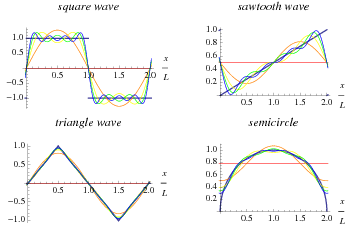
\includegraphics{FourierSeriesExamples_800.png}
\end{center}
Using the method for a generalized Fourier series, the usual Fourier series involving sines and cosines is obtained by taking $f_1(x)=cosx$ and $f_2(x)=sinx$. Since these functions form a complete orthogonal system over $[-\pi,\pi]$, the Fourier series of a function $f(x)$ is given by (with $n\in \mathbb{N}$)
\begin{align}
f(x)&=\frac{1}{2}a_0+\sum_{i=1}^{\infty}a_n\cos(nx)+\sum_{i=1}^{\infty}b_n\sin(nx) \\
a_0&= \frac{1}{\pi} \int_{-\pi}^{\pi}f(x)dx \\
a_n&= \frac{1}{\pi} \int_{-\pi}^{\pi}f(x)\cos(nx)dx \\
b_n&= \frac{1}{\pi} \int_{-\pi}^{\pi}f(x)\sin(nx)dx.
\end{align}
For a function f(x) periodic on an interval [-L,L] instead of [-pi,pi], a simple change of variables can be used to transform the interval of integration from [-pi,pi] to [-L,L]. Let 
\begin{align}
x &\equiv \frac{\pi x'}{L} \implies x'=\frac{Lx}{\pi} \\
dx &= \frac{\pi dx'}{L}.
\end{align}
\end{defn}
In Physics, Fourier series play a large part in representing physical systems. Any periodic function with period $\tau$ can be written as a sum of sine and cosine terms. Very similar to above, yet slightly different, we can write
\begin{align}
f(t)&=\sum_{n=0}^{\infty}[a_n\cos(n\omega t)+b_n\sin(n\omega t)] \\
a_n&= \frac{2}{\tau}\int_{-\tau/2}^{\tau/2}f(t)\cos(n\omega t)dt \hspace{2cm} [n \geq 1] \\
b_n&= \frac{2}{\tau}\int_{-\tau/2}^{\tau/2}f(t)\sin(n\omega t)dt \hspace{2cm} [n \geq 1] \\
a_0&= \frac{1}{\tau}\int_{-\tau/2}^{\tau/2}f(t)dt.
\end{align}
Since we know the period is $\tau$, we can establish a relationship between $\tau$ and $\omega$. By definition, $\tau=1/f$, where $f$ is the frequency of our system. We then have $\omega=2\pi f$, which allows us to say $f=\frac{\omega}{2\pi}\implies \tau=\frac{2\pi}{\omega}$. It is sometimes useful to express a Fourier series as an exponential
\begin{align}
f(t)=\sum_{n=-\infty}^{\infty}A_ne^{in\omega t}.
\end{align} 
If we analyze this form, we can see that it is equivalent to the sine and cosine form. First, notice that we are summing all terms over the interval $(-\infty, \infty)$, which means we can immediately separate this into multiple sums such as
\begin{align}
f(t)=A_0+\sum_{n=1}^{\infty}A_ne^{in\omega t}+\sum_{n=1}^{\infty}A_{-n}e^{-in\omega t}.
\end{align}
Since we are defining out summation limits as the same for both sums in the above expression, this can also be written as
\begin{align}
f(t)=A_0+\sum_{n=1}^{\infty}\big(A_ne^{in\omega t}+A_{-n}e^{-in\omega t}\big).
\end{align}
If we then want to consider only the real possible functions, we can use Euler's identity $e^{i\theta}=\cos(\theta)+i\sin(\theta)$ to derive the conditions on $A_n$ and $A_{-n}$. Since we know each exponential will have an imaginary part, it must be true also that each coefficient will also have an imaginary part in order for the total function to become real; in other words, they will be complex coefficients. Let the real part of each coefficient be denoted by $\mathfrak{R}(A_n)$ and the imaginary part as $\mathfrak{I}(A_n)$. Then we have $A_n=\mathfrak{R}(A_n)+i\mathfrak{I}(A_n)$ for all $n$. Since we want $f(t)$ to be real, each part of it must be real, therefore, we can immediately let $A_0$ be real and then only worry about the other $A_n$ terms when $n\neq 0$. From this, we can say equation (5.13) becomes
\begin{align}
f(t)=A_0+\sum_{n=1}^{\infty}\big(A_n\big[\cos(n\omega t)+i\sin(n\omega t)\big]+A_{-n}\big[\cos(-n\omega t)+i\sin(-n\omega t)\big]\big).
\end{align}
It is also important to know that $\cos(-\theta)=\cos(\theta)$ and $\sin(-\theta)=-\sin(\theta)$. From here, we can say
\begin{align}
f(t)&=A_0+\sum_{n=1}^{\infty}\big(A_n\big[\cos(n\omega t)+i\sin(n\omega t)\big]+A_{-n}\big[\cos(in\omega t)-i\sin(n\omega t)\big]\big)\\
&=A_0+\sum_{n=1}^{\infty}\big([A_n+A_{-n}]\cos(n\omega t)+[A_n-A_{-n}]i\sin(n\omega t)\big).
\end{align}
Now, if we express the coefficients in terms of their real and imaginary terms, we get
\begin{align}
f(t)&=A_0+\sum_{n=1}^{\infty}\bigg(\big[\mathfrak{R}(A_n)+\mathfrak{R}(A_{-n})+i\mathfrak{I}(A_n)+i\mathfrak{I}(A_{-n})\big]\cos(n\omega t) \nonumber \\&\hspace{1.1cm}+\big[\mathfrak{R}(A_n)-\mathfrak{R}(A_{-n})+i\mathfrak{I}(A_n)-i\mathfrak{I}(A_{-n})\big]i\sin(n\omega t)\bigg) \\
&=A_0+\sum_{n=1}^{\infty}\bigg(\big[\mathfrak{R}(A_n)+\mathfrak{R}(A_{-n})+i\mathfrak{I}(A_n)+i\mathfrak{I}(A_{-n})\big]\cos(n\omega t) \nonumber \\&\hspace{1.1cm}+\big[i\mathfrak{R}(A_n)-i\mathfrak{R}(A_{-n})-\mathfrak{I}(A_n)+\mathfrak{I}(A_{-n})\big]\sin(n\omega t)\bigg).
\end{align}
From here, we can ignore the real parts and isolate the imaginary parts that we want to cancel out. One possible way to make this real, is if all of the imaginary parts sum to zero. We can easily show that $\sum a+b=\sum a+\sum b$, which means we can separate just the imaginary summation and equate it to zero, leaving our $f(t)$ as all real terms. This gives us
\begin{align}
0=\sum_{n=1}^{\infty}\bigg(\big[i\mathfrak{I}(A_n)+i\mathfrak{I}(A_{-n})\big]\cos(n\omega t)+\big[i\mathfrak{R}(A_n)-i\mathfrak{R}(A_{-n})]\sin(n\omega t)\bigg).
\end{align}
If we have every term equate to zero, we know that entire sum will equate to zero. Therefore, we can solve for our $n$ dependent coefficients that will make each term zero, and this will give us the solution to make the entire sum zero. Since we have a sine and a cosine term in each separate $n$ term of the sum, we can then make each one zero by setting the coefficients in front of the respective term zero. This then gives us a set of equations
\begin{align}
0 &=i\mathfrak{I}(A_n)+i\mathfrak{I}(A_{-n}) \\
0 &=i\mathfrak{R}(A_n)-i\mathfrak{R}(A_{-n}).
\end{align}
From here we simply get
\begin{align}
\mathfrak{I}(A_n)&=-\mathfrak{I}(A_{-n}) \\
\mathfrak{R}(A_n)&=\mathfrak{R}(A_{-n}).
\end{align}
This tells us that the real component of $A_n$ and $A_{-n}$ are equivalent, and the imaginary component of $A_n$ is the negative of the respective component in $A_{-n}$. Since $n$ is generic, we can conclude that $A_n$ is the conjugate of $A_{-n}$ for all $n\neq0$, or
\begin{align}
\mathfrak{R}(A_n)+i\mathfrak{I}(A_n)=\mathfrak{R}(A_{-n})-i\mathfrak{I}(A_{-n})  \implies A_n=A^*_{-n}.
\end{align} 
Thus, we have determined that for our Fourier series to be real, we must have $A_n=A^*_{-n}$. Furthermore, we can combine equations (5.22), (5.23) and (5.18) so say
\begin{align}
f(t)&=A_0+\sum_{n=1}^{\infty}\bigg(\big[\mathfrak{R}(A_n)+\mathfrak{R}(A_{n})+i\mathfrak{I}(A_n)-i\mathfrak{I}(A_{n})\big]\cos(n\omega t) \nonumber \\&\hspace{1.1cm}+\big[i\mathfrak{R}(A_n)-i\mathfrak{R}(A_{n})-\mathfrak{I}(A_n)-\mathfrak{I}(A_{n})\big]\sin(n\omega t)\bigg) \\
&=A_0+\sum_{n=1}^{\infty}\bigg(\big[\mathfrak{R}(A_n)+\mathfrak{R}(A_{n})\big]\cos(n\omega t) +\big[-\mathfrak{I}(A_n)-\mathfrak{I}(A_{n})\big]\sin(n\omega t)\bigg) \\
&=A_0+\sum_{n=1}^{\infty}\bigg(2\mathfrak{R}(A_n)\cos(n\omega t) -2\mathfrak{I}(A_n)\sin(n\omega t)\bigg).
\end{align} 
From here, letting $a_n=2\mathfrak{R}(A_n)$ and $b_n=-2\mathfrak{I}(A_n)$, we get
\begin{align}
f(t)&=A_0+\sum_{n=1}^{\infty}\bigg(a_n\cos(n\omega t) +b_n\sin(n\omega t)\bigg) \\
&=A_0+\sum_{n=1}^{\infty}a_n\cos(n\omega t) +\sum_{n=1}^{\infty}b_n\sin(n\omega t).
\end{align}
Thus, as we can see from above, this is of the same form as equation (5.7), so we have verified that the exponential form of the Fourier series is equivalent to the sine and cosine form. The constants $A_0$, $a_n$ and $b_n$ can be solved from here using equations (5.8) through (5.10). Using (5.9) and (5.10), we can solve for the $A_n$ from equation (5.11). First we know $a_n=2\mathfrak{R}(A_n)$ and $b_n=-2\mathfrak{I}(A_n)$ so we can say
\begin{align}
a_n&= \frac{2}{\tau}\int_{-\tau/2}^{\tau/2}f(t)\cos(n\omega t)dt=2\mathfrak{R}(A_n)\\
b_n&= \frac{2}{\tau}\int_{-\tau/2}^{\tau/2}f(t)\sin(n\omega t)dt=-2\mathfrak{I}(A_n).
\end{align}
Simplifying this, we have
\begin{align}
\mathfrak{R}(A_n)&=\frac{1}{\tau}\int_{-\tau/2}^{\tau/2}f(t)\cos(n\omega t)dt \\
\mathfrak{I}(A_n)&=-\frac{1}{\tau}\int_{-\tau/2}^{\tau/2}f(t)\sin(n\omega t)dt.
\end{align}
From these, we can write 
\begin{align}
A_n&=\mathfrak{R}(A_n)+i\mathfrak{I}(A_n)\\ &=\frac{1}{\tau}\int_{-\tau/2}^{\tau/2}f(t)\cos(n\omega t)dt-\frac{i}{\tau}\int_{-\tau/2}^{\tau/2}f(t)\sin(n\omega t)dt \\
&= \frac{1}{\tau}\int_{-\tau/2}^{\tau/2}\big[f(t)\cos(n\omega t)-f(t)i\sin(n\omega t)\big]dt \\
&= \frac{1}{\tau}\int_{-\tau/2}^{\tau/2}f(t)\big[\cos(-n\omega t)+i\sin(-n\omega t)\big]dt \\
&=\frac{1}{\tau}\int_{-\tau/2}^{\tau/2}f(t)e^{-in\omega t}dt.
\end{align}
Notice that $A_0=a_0$ from comparing equations (5.7) and (5.29). Also, if we let $n=0$ in equation (5.38), we get 
\begin{align}
A_0&=\frac{1}{\tau}\int_{-\tau/2}^{\tau/2}f(t)dt \\
&= a_0.
\end{align}
Thus, we can see that we do not have to separate $A_0$ from the exponential form of our Fourier series as $A_0$ equates to $a_0$ which can be directly derived from (5.38). Therefore, we can simply say
\begin{defn}[Exponential Fourier Series]{FourierSeries2}
	A Fourier series can be expressed as an infinite sum of exponentials from
	\begin{align}
	f(t)=\sum_{n=-\infty}^{\infty}A_ne^{in\omega t}\hspace{1cm}\textrm{with}\hspace{1cm}
	A_n=\frac{1}{\tau}\int_{-\tau/2}^{\tau/2}f(t)e^{-in\omega t}dt
	\end{align}
\end{defn}
An alternate derivation for $A_n$ can be quickly and directly discovered from equation (5.11). First, we can multiple by $e^{-in\omega t}$ to get
\begin{align}
f(t)e^{-imwt}=\sum_{n=-\infty}^{\infty}A_ne^{in\omega t}e^{-im \omega t}.
\end{align}
Next, multiplying by $dt$ then taking the integral of both sides of this expression over one period $\tau$ gives us
\begin{align}
\int_{-\tau/2}^{\tau/2}f(t)e^{-im\omega t}dt&=\int_{-\tau/2}^{\tau/2}\sum_{n=-\infty}^{\infty}A_ne^{in\omega t}e^{-im\omega t}dt.
\end{align}
Since, each $A_n$ term is a constant, then their sum will also be a constant and thus we can say
\begin{align}
\int_{-\tau/2}^{\tau/2}f(t)e^{-imwt}dt&=\sum_{n=-\infty}^{\infty}A_n\int_{-\tau/2}^{\tau/2}e^{i(n-m)\omega t}dt.
\end{align}
Evaluating this integral can be done by using Eulers formula. Let us denote it separately by $g(t)$. It follows
\begin{align}
g(t)=\int_{-\tau/2}^{\tau/2}e^{i(n-m)\omega t}dt=\int_{-\tau/2}^{\tau/2}\big[\cos((n-m)\omega t)+i\sin((n-m)\omega t) \big]dt.
\end{align}
Since we are only worried about the real part for now while integrating, we can simplify this further to
\begin{align}
g(t)=\int_{-\tau/2}^{\tau/2}\cos((n-m)\omega t)dt.
\end{align}
From here, if we let $u=(n-m)\omega t$, then $du=(n-m)\omega dt$, which gives us
\begin{align}
g(t)&=\int_{-\tau/2}^{\tau/2}\frac{\cos(u)du}{(n-m)\omega}\\ &=\frac{\sin(u)}{(n-m)\omega}\bigg]_{-\tau/2}^{\tau/2} \\
&=\frac{\sin((n-m)\omega t)}{(n-m)\omega}\bigg]_{-\tau/2}^{\tau/2} \\
&=\frac{\sin((n-m)\omega (\tau/2))}{(n-m)\omega}-\frac{\sin((n-m)\omega (-\tau/2))}{(n-m)\omega} \\
&=\frac{\sin((n-m)\omega (\tau/2))}{(n-m)\omega}+\frac{\sin((n-m)\omega (\tau/2))}{(n-m)\omega} \\
&=\frac{2\sin((n-m)\omega (\tau/2))}{(n-m)\omega}.
\end{align}
Since $\tau=\frac{2\pi}{\omega} \implies \omega = \frac{2\pi}{\tau}$, this then becomes
\begin{align}
g(t)=\frac{\tau\sin((n-m)\pi))}{(n-m)\pi}.
\end{align}
We can notice that for all values of $n$ and $m$ ($n\neq m$), $n-m$ will be an integer, since $n,m\in\mathbb{Z}$. This means, that for all values of n and m ($n\neq m$), we will have $g(t)=0$. The only exception to this is when $n=m$. In this case we have the indeterminate form and instead can evaluate $g(t)$ by taking the limit as $n$ approaches $m$ and using L'Hospital's rule. This gives
\begin{align}
g(t)&=\lim\limits_{n\rightarrow m}\frac{\tau\sin((n-m)\pi))}{(n-m)\pi} \\
&=\lim\limits_{n\rightarrow m}\frac{d/dn}{d/dn}\frac{\tau\sin((n-m)\pi))}{(n-m)\pi} \\
&=\lim\limits_{n\rightarrow m}\frac{\tau\pi\cos((n-m)\pi)}{\pi}\\
&=\tau\cos(0) \\
&=\tau.
\end{align}
Combining this with equation (5.44) will then give us an integral for deriving $A_n$. First, notice that because the integral evaluates to zero for all $n\neq m$ terms, each term of our sum over $\mathbb{R}$ will be zero except when $m=n$. Thus, (5.44) becomes
\begin{align}
\int_{-\tau/2}^{\tau/2}f(t)e^{-im \omega t}dt&=A_m\tau.
\end{align}
Finally, dividing by $\tau$ gives us
\begin{align}
A_m=\frac{1}{\tau}\int_{-\tau/2}^{\tau/2}f(t)e^{-imwt}dt,
\end{align}
which is equivalent to (5.38). 








\newpage
\section{Schr\"{o}dinger's Equation}
A perfect example of a differential equation is the schr\"{o}dinger Equation (SE). 
\begin{defn}[Schr\"{o}dinger equation (Taken from http://scienceworld.wolfram.com)]{1}
	 The Schrödinger equation is the fundamental equation of physics for describing quantum mechanical behavior. It is also often called the Schrödinger wave equation, and is a partial differential equation that describes how the wavefunction of a physical system evolves over time. The time-dependent one-dimensional Schrödinger equation is given by 
	 \begin{align*}
	 i\hbar\frac{\partial \Psi}{\partial t}=-\frac{\hbar^2}{2m}\frac{\partial^2 \Psi}{\partial x^2}+V(x)\Psi(x,t)\equiv \hat{H}\Psi(x,t).
	 \end{align*}
\end{defn}
This equation is used very often in physics. Let us explore it a bit. First, let us consider a simple wave of the form $\Psi(x,t)=Ae^{i(kx-\omega t)}$. Taking the respective derivatives with respect to $t$ and $x$ gives us $\frac{\partial \Psi}{\partial t}=-i\omega Ae^{i(kx-\omega t)}$ and $\frac{\partial^2 \Psi}{\partial x^2}=-k^2 Ae^{i(kx-\omega t)}$. From here, inserting them into the Schr\"{o}dinger equation gives us
\begin{align}
i\hbar\big(-i\omega Ae^{i(kx-\omega t)} \big)=-\frac{\hbar^2}{2m}\big(-k^2 Ae^{i(kx-\omega t)} \big)+V(x)\big(Ae^{i(kx-\omega t)} \big).
\end{align}
Dividing out $Ae^{i(kx-\omega t)}$ and simplifying this gives us
\begin{align}
\hbar\omega=\frac{\hbar^2k^2}{2m}+V(x).
\end{align}
Now, $\hbar$ which is the reduced Plancks costant is equivalent to $\frac{h}{2\pi}$, $k=\frac{2\pi}{\lambda}$ and $p=\frac{h}{\lambda}$. Combining these with (7.2) allows us to verify this is a solution. First, $E=\hbar \omega$ and $KE=\frac{p^2}{2m}$ allows us to see
\begin{align}
\hbar\omega=\frac{\hbar^2k^2}{2m}+V(x) \Longleftrightarrow \hbar\omega=\frac{p^2}{2m}+V(x) \Longleftrightarrow E=KE+PE,
\end{align}
which is the conservation of energy. Hence since we know this to be true for any closed system, we have verified that a general wave of the form $\Psi(x,t)=Ae^{i(kx-\omega t)}$ is a solution to the SE. A periodic wave can be constructed from a sum of plane waves
\begin{align}
\psi(x,t) &= \sum_{i=1}^{n} A_i \cos(k_ix_i-\omega_i t).
\end{align}










%%%%%%%%%%%%%%%%%%%%%%%%%%%%%%%%%%%%%%%%%%%%%%%%%%%%%%%%%%%%%%%%%%%%%%%%%%%%%%%%%%%%%%%%%%%

%%%%%%%%%%%%%%%%%%%%%%%%%%%%%%%%%%%%%%%%%%%%%%%%%%%%%%%%%%%%%%%%%%%%%%%%%%%%%%%%%%%%%%%%%%%
\end{document}